\documentclass[tikz, margin = 1cm]{standalone}
\usepackage{mathtools}
\usepackage{amsmath}
\usepackage{pgfplots}
\pgfplotsset{compat=1.8}


% IMPORT-DATA beryll_raw data/beryll_result
% IMPORT-DATA elbait_raw data/elbait_result
% IMPORT-DATA gateway_raw data/gateway_result
% IMPORT-DATA saphir_raw data/saphir_result
% IMPORT-DATA snail03_raw data/snail03_result
% IMPORT-DATA snail04_raw data/snail04_result
% IMPORT-DATA snail05_raw data/snail05_result

%% SQL CREATE TABLE beryll AS
%% SELECT 0 AS x_base, * FROM beryll_raw;

%% SQL CREATE TABLE elbait AS
%% SELECT 3 AS x_base, * FROM elbait_raw;

%% SQL CREATE TABLE gateway AS
%% SELECT 6 AS x_base, * FROM gateway_raw;

%% SQL CREATE TABLE saphir AS
%% SELECT 1 AS x_base, * FROM saphir_raw;

%% SQL CREATE TABLE snail03 AS
%% SELECT 5 AS x_base, * FROM snail03_raw;

%% SQL CREATE TABLE snail04 AS
%% SELECT 4 AS x_base, * FROM snail04_raw;

%% SQL CREATE TABLE snail05 AS
%% SELECT 2 AS x_base, * FROM snail05_raw;

%% SQL CREATE TABLE merged_raw AS
%% SELECT * FROM beryll UNION ALL 
%% SELECT * FROM elbait UNION ALL 
%% SELECT * FROM gateway UNION ALL 
%% SELECT * FROM saphir UNION ALL 
%% SELECT * FROM snail03 UNION ALL
%% SELECT * FROM snail04 UNION ALL 
%% SELECT * FROM snail05

%% SQL CREATE TABLE merged AS
%% SELECT 0, x_base * 12 + LOG(n) / LOG(2) - 20 AS x, * FROM merged_raw
%% ORDER BY x


\pgfplotsset{seq1/.style={gray, mark=none}}
\pgfplotsset{seq/.style={seq1, forget plot}}

\pgfplotsset{rand1/.style={gray, mark=triangle}}
\pgfplotsset{rand/.style={rand1, forget plot}}

\pgfplotsset{split1/.style={blue, mark=o}}
\pgfplotsset{split/.style={split1, forget plot}}

\pgfplotsset{joint1/.style={red, mark=*}}
\pgfplotsset{joint/.style={joint1, forget plot}}

\newcommand{\leftlabel}[1]{$\ \ \ 2^{23}\mathrlap{\quad\ \underset{\clap{\normalsize\bfseries#1}}{\strut}}$}
\newcommand{\rightlabel}{$2^{30}\ \ \ $}

\begin{document}

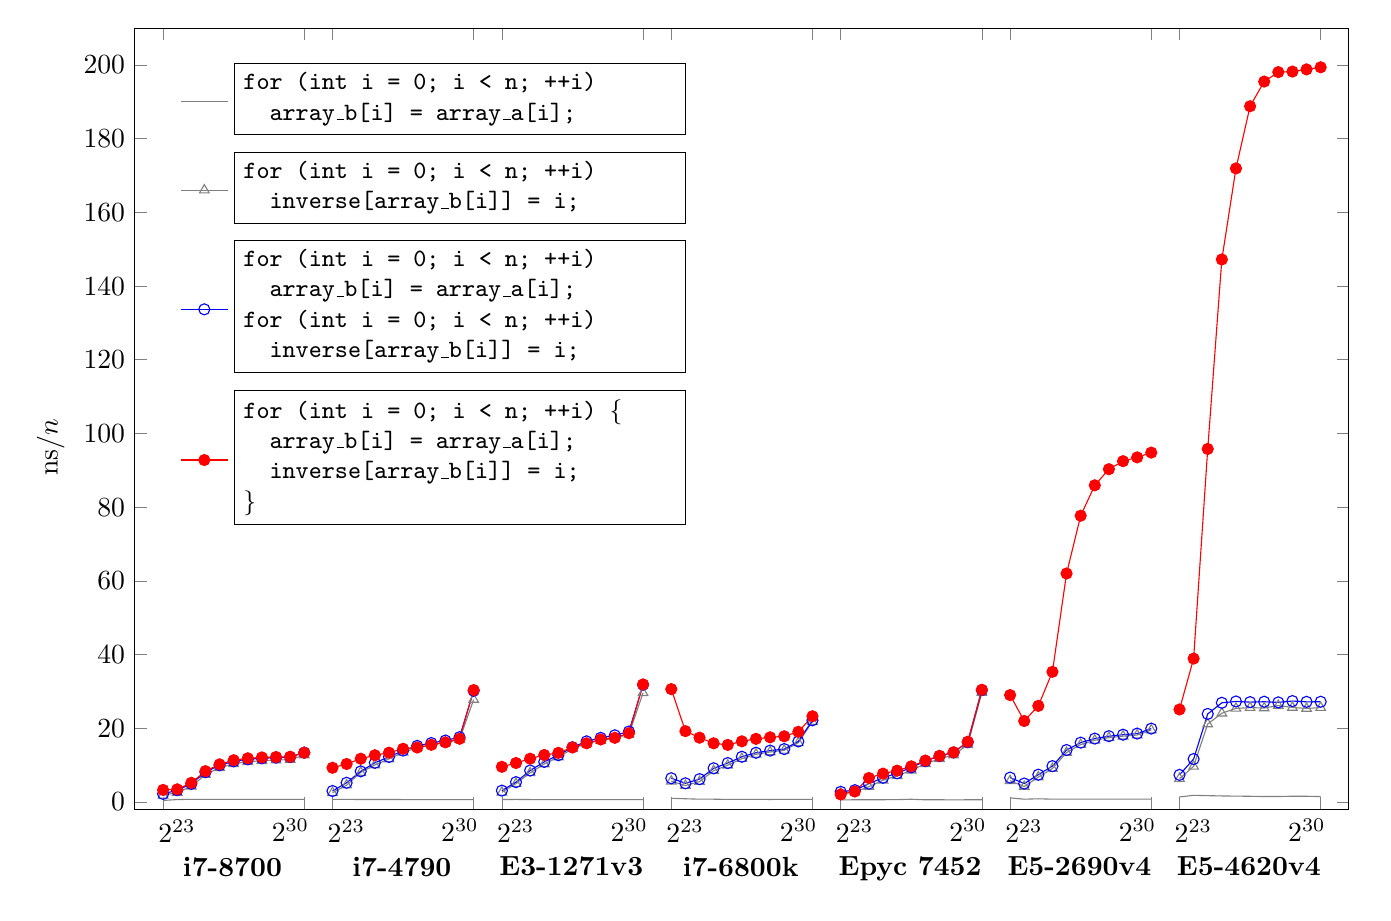
\begin{tikzpicture}
\begin{axis}[
	at = {(0,0)},
	anchor = south west,
    ymin = -2,
    ymax = 210,
    xmin = -2,
    xmax = 84,
    width = 17cm,
    height = 11.5cm,
    ylabel={\llap{$\textnormal{ns} / n$}},
    xtick={0,10,12,22,24,34,36,46,48,58,60,70,72,82},
    xticklabels={%
    \leftlabel{i7-8700},\rightlabel,
    \leftlabel{i7-4790},\rightlabel,
    \leftlabel{E3-1271v3},\rightlabel,
    \leftlabel{i7-6800k},\rightlabel,
    \leftlabel{Epyc 7452},\rightlabel,
    \leftlabel{E5-2690v4},\rightlabel,
    \leftlabel{E5-4620v4},\rightlabel,
    },
    %y label style={rotate=270},
    legend pos=north west,
    legend cell align={left},
    legend columns=4,
    transpose legend,
    legend style={draw=none, font=\small},
    ]
    
    
    
%% MULTIPLOT(x_base)
%% SELECT 1000.0 * seq / n AS y, * FROM merged
\addplot[seq1] coordinates { (0.0,0.379562) (1.0,0.618935) (2.0,0.687122) (3.0,0.680447) (4.0,0.674546) (5.0,0.675231) (6.0,0.671461) (7.0,0.671163) (8.0,0.667404) (9.0,0.668267) (10.0,0.669764) };
\addlegendentry{x\_base=0};
\addplot[seq] coordinates { (12.0,0.646591) (13.0,0.671387) (14.0,0.629902) (15.0,0.622153) (16.0,0.627935) (17.0,0.619203) (18.0,0.613943) (19.0,0.614651) (20.0,0.615157) (21.0,0.615204) (22.0,0.614946) };
\addlegendentry{x\_base=1};
\addplot[seq] coordinates { (24.0,0.619888) (25.0,0.652313) (26.0,0.620127) (27.0,0.613093) (28.0,0.601709) (29.0,0.59849) (30.0,0.596195) (31.0,0.594832) (32.0,0.595987) (33.0,0.595687) (34.0,0.594887) };
\addlegendentry{x\_base=2};
\addplot[seq] coordinates { (36.0,0.965118) (37.0,0.834942) (38.0,0.718355) (39.0,0.71764) (40.0,0.658154) (41.0,0.653833) (42.0,0.66331) (43.0,0.646397) (44.0,0.659216) (45.0,0.656577) (46.0,0.669052) };
\addlegendentry{x\_base=3};
\addplot[seq] coordinates { (48.0,0.523567) (49.0,0.561237) (50.0,0.555992) (51.0,0.576019) (52.0,0.607252) (53.0,0.703126) (54.0,0.55483) (55.0,0.555068) (56.0,0.546727) (57.0,0.554133) (58.0,0.556995) };
\addlegendentry{x\_base=4};
\addplot[seq] coordinates { (60.0,1.07193) (61.0,0.717163) (62.0,0.82612) (63.0,0.727534) (64.0,0.729144) (65.0,0.725538) (66.0,0.726163) (67.0,0.726327) (68.0,0.725813) (69.0,0.725824) (70.0,0.726424) };
\addlegendentry{x\_base=5};
\addplot[seq] coordinates { (72.0,1.33133) (73.0,1.76668) (74.0,1.68109) (75.0,1.59788) (76.0,1.55073) (77.0,1.50749) (78.0,1.43965) (79.0,1.44465) (80.0,1.52002) (81.0,1.51136) (82.0,1.42589) };
\addlegendentry{x\_base=6};


    
    
%% MULTIPLOT(x_base)
%% SELECT 1000.0 * rand / n AS y, * FROM merged
\addplot[rand1] coordinates { (0.0,1.77765) (1.0,2.54583) (2.0,4.18425) (3.0,7.37727) (4.0,9.25189) (5.0,10.3146) (6.0,10.8843) (7.0,11.1575) (8.0,11.3267) (9.0,11.4715) (10.0,12.6929) };
\addlegendentry{x\_base=0};
\addplot[rand] coordinates { (12.0,2.48146) (13.0,4.53043) (14.0,7.97606) (15.0,10.0096) (16.0,11.6434) (17.0,13.4442) (18.0,14.7096) (19.0,15.4295) (20.0,16.0503) (21.0,16.9392) (22.0,27.7729) };
\addlegendentry{x\_base=1};
\addplot[rand] coordinates { (24.0,2.58446) (25.0,4.9448) (26.0,7.86066) (27.0,10.2738) (28.0,12.1785) (29.0,14.3801) (30.0,15.8603) (31.0,16.638) (32.0,17.2989) (33.0,18.3071) (34.0,29.6177) };
\addlegendentry{x\_base=2};
\addplot[rand] coordinates { (36.0,5.59902) (37.0,4.41599) (38.0,5.4853) (39.0,8.45802) (40.0,9.93955) (41.0,11.7348) (42.0,12.8942) (43.0,13.5349) (44.0,13.9609) (45.0,16.0293) (46.0,21.8181) };
\addlegendentry{x\_base=3};
\addplot[rand] coordinates { (48.0,2.36416) (49.0,2.69079) (50.0,4.11606) (51.0,5.86796) (52.0,7.06166) (53.0,8.56477) (54.0,10.3325) (55.0,11.7008) (56.0,12.7005) (57.0,15.5091) (58.0,29.6375) };
\addlegendentry{x\_base=4};
\addplot[rand] coordinates { (60.0,5.72395) (61.0,4.1647) (62.0,6.71124) (63.0,9.03499) (64.0,13.3831) (65.0,15.5455) (66.0,16.7072) (67.0,17.4343) (68.0,17.8205) (69.0,18.1308) (70.0,19.4813) };
\addlegendentry{x\_base=5};
\addplot[rand] coordinates { (72.0,6.29997) (73.0,9.62639) (74.0,21.1232) (75.0,24.0517) (76.0,25.3697) (77.0,25.5711) (78.0,25.4638) (79.0,26.142) (80.0,25.6257) (81.0,25.3437) (82.0,25.5973) };
\addlegendentry{x\_base=6};

    
%% MULTIPLOT(x_base)
%% SELECT 1000.0 * split / n AS y, * FROM merged
\addplot[split1] coordinates { (0.0,2.15054) (1.0,3.15475) (2.0,4.87089) (3.0,8.04996) (4.0,9.93115) (5.0,10.9927) (6.0,11.565) (7.0,11.831) (8.0,11.9923) (9.0,12.1538) (10.0,13.3697) };
\addlegendentry{x\_base=0};
\addplot[split] coordinates { (12.0,2.93732) (13.0,5.1775) (14.0,8.2705) (15.0,10.5983) (16.0,12.1836) (17.0,13.9143) (18.0,15.191) (19.0,15.96) (20.0,16.6471) (21.0,17.5499) (22.0,30.1425) };
\addlegendentry{x\_base=1};
\addplot[split] coordinates { (24.0,3.04317) (25.0,5.35154) (26.0,8.50129) (27.0,10.8466) (28.0,12.6613) (29.0,14.8259) (30.0,16.4212) (31.0,17.3739) (32.0,18.0588) (33.0,19.0908) (34.0,31.7867) };
\addlegendentry{x\_base=2};
\addplot[split] coordinates { (36.0,6.4106) (37.0,5.03445) (38.0,6.16121) (39.0,9.1145) (40.0,10.5258) (41.0,12.2343) (42.0,13.3274) (43.0,13.9039) (44.0,14.3232) (45.0,16.4005) (46.0,22.1205) };
\addlegendentry{x\_base=3};
\addplot[split] coordinates { (48.0,2.72846) (49.0,3.16525) (50.0,4.93956) (51.0,6.53994) (52.0,7.76231) (53.0,9.34365) (54.0,11.0482) (55.0,12.4371) (56.0,13.4037) (57.0,16.204) (58.0,30.3287) };
\addlegendentry{x\_base=4};
\addplot[split] coordinates { (60.0,6.58035) (61.0,4.96244) (62.0,7.37143) (63.0,9.69529) (64.0,14.0692) (65.0,16.0708) (66.0,17.1705) (67.0,17.8293) (68.0,18.2234) (69.0,18.5288) (70.0,19.8773) };
\addlegendentry{x\_base=5};
\addplot[split] coordinates { (72.0,7.3185) (73.0,11.6148) (74.0,23.8597) (75.0,26.8824) (76.0,27.2446) (77.0,27.0739) (78.0,27.1733) (79.0,26.999) (80.0,27.3586) (81.0,27.1424) (82.0,27.1673) };
\addlegendentry{x\_base=6};
    
    
%% MULTIPLOT(x_base)
%% SELECT 1000.0 * joint / n AS y, * FROM merged
\addplot[joint1] coordinates { (0.0,3.23868) (1.0,3.39365) (2.0,5.15962) (3.0,8.33356) (4.0,10.1833) (5.0,11.303) (6.0,11.8203) (7.0,12.0625) (8.0,12.1654) (9.0,12.2364) (10.0,13.3361) };
\addlegendentry{x\_base=0};
\addplot[joint] coordinates { (12.0,9.24587) (13.0,10.2744) (14.0,11.6999) (15.0,12.6511) (16.0,13.3474) (17.0,14.4078) (18.0,14.7467) (19.0,15.4768) (20.0,16.1487) (21.0,17.1159) (22.0,30.3429) };
\addlegendentry{x\_base=1};
\addplot[joint] coordinates { (24.0,9.50718) (25.0,10.5391) (26.0,11.7204) (27.0,12.7186) (28.0,13.2981) (29.0,14.7706) (30.0,15.8912) (31.0,16.9293) (32.0,17.38) (33.0,18.625) (34.0,31.8669) };
\addlegendentry{x\_base=2};
\addplot[joint] coordinates { (36.0,30.5958) (37.0,19.1913) (38.0,17.4191) (39.0,15.8893) (40.0,15.4587) (41.0,16.4239) (42.0,17.0986) (43.0,17.5124) (44.0,17.7867) (45.0,19.0102) (46.0,23.2323) };
\addlegendentry{x\_base=3};
\addplot[joint] coordinates { (48.0,1.99986) (49.0,2.80428) (50.0,6.47807) (51.0,7.65836) (52.0,8.46952) (53.0,9.63888) (54.0,11.2057) (55.0,12.4789) (56.0,13.4393) (57.0,16.3205) (58.0,30.4152) };
\addlegendentry{x\_base=4};
\addplot[joint] coordinates { (60.0,28.9783) (61.0,21.9455) (62.0,26.0518) (63.0,35.3019) (64.0,61.9832) (65.0,77.6737) (66.0,85.9217) (67.0,90.3044) (68.0,92.4779) (69.0,93.5035) (70.0,94.8001) };
\addlegendentry{x\_base=5};
\addplot[joint] coordinates { (72.0,25.074) (73.0,38.8837) (74.0,95.7904) (75.0,147.233) (76.0,171.94) (77.0,188.819) (78.0,195.52) (79.0,198.084) (80.0,198.229) (81.0,198.829) (82.0,199.397) };
\addlegendentry{x\_base=6};



\legend{
{\parbox{6cm}{\fbox{\parbox{5.5cm}{%
\texttt{for (int i = 0; i < n; ++i)}\\
\texttt{\textcolor{white}{.}\ array\_b[i] = array\_a[i];}
}}\\\\\\}},
{\parbox{6cm}{\fbox{\parbox{5.5cm}{%
\texttt{for (int i = 0; i < n; ++i)}\\
\texttt{\textcolor{white}{.}\ inverse[array\_b[i]] = i;}%
}}\\\\\\}},
{\parbox{6cm}{\fbox{\parbox{5.5cm}{%
\texttt{for (int i = 0; i < n; ++i)}\\
\texttt{\textcolor{white}{.}\ array\_b[i] = array\_a[i];}\\
\texttt{for (int i = 0; i < n; ++i)}\\
\texttt{\textcolor{white}{.}\ inverse[array\_b[i]] = i;}%
}}\\\\\\\\\\}},
{\parbox{6cm}{\fbox{\parbox{5.5cm}{%
\texttt{for (int i = 0; i < n; ++i) \{}\\
\texttt{\textcolor{white}{.}\ array\_b[i] = array\_a[i];}\\
\texttt{\textcolor{white}{.}\ inverse[array\_b[i]] = i;}\\
\texttt{\}}
}}\\\\\\\\\\}},}
\end{axis}

\end{tikzpicture}

\end{document}
